\subsubsection{Simulation service}
\textbf{Overview}

\texttt{SimulationService} is a high-performance distributed simulation management system designed to orchestrate, execute, and monitor simulation tasks across a computational cluster. The service provides a robust API for transferring simulation models, processing requests, and managing the lifecycle of the simulation infrastructure.

\bigskip
\textbf{Architecture}

The service is built on a client-server architecture using gRPC for high-performance communication. It leverages a worker pool pattern to distribute simulation workloads efficiently across available computational resources. \texttt{SimulationService} system architecture is present in Fig. \ref{fig:SimulationServiceSystemArchitecture}.

\bigskip
\textbf{System Components}

\bigskip
Main system components:

\begin{itemize}
	\item \textbf{Simulation Service} - main service class, where user or optimization system reach simulation cluster

	\item \textbf{Server} - Central coordinator of the simulation cluster, build from dedicated \textit{Dockerfile}. Launched as \textit{Docker container} via \textit{Docker compose}. Communication between \textbf{Simulation Service} and \textbf{Worker(s)} are handled using gRPC protocol.

	Responsibilities:
	\begin{itemize}
		\item Accepts simulation model uploads
		\item Distributes simulation jobs to available workers
		\item Tracks simulation progress and collects results
		\item Maintains state about connected workers and available models
	\end{itemize}

	\item \textbf{Worker Pool} - Compute nodes responsible for executing simulation jobs. Built from a \textit{Dockerfile}. Can be replicated (N instances) to scale horizontally. Initialized on cluster start and shut down on cluster termination.
		Responsibilities:
	\begin{itemize}
		\item Connect to the server and introduce themselves.
		\item Retrieve the simulation model from the server.
		\item Poll for simulation jobs.
		\item Perform simulations using the provided model and case data.
		\item Return simulation results to the server.
	\end{itemize}

\end{itemize}

\begin{figure}[H]
	\centering
	\includegraphics[width=1.0\textwidth]{content/images/SimulationServiceArchitecture.pdf}
	\caption{Simulation service system architecture}
	\label{fig:SimulationServiceSystemArchitecture}
\end{figure}

\begin{figure}[H]
	\centering
	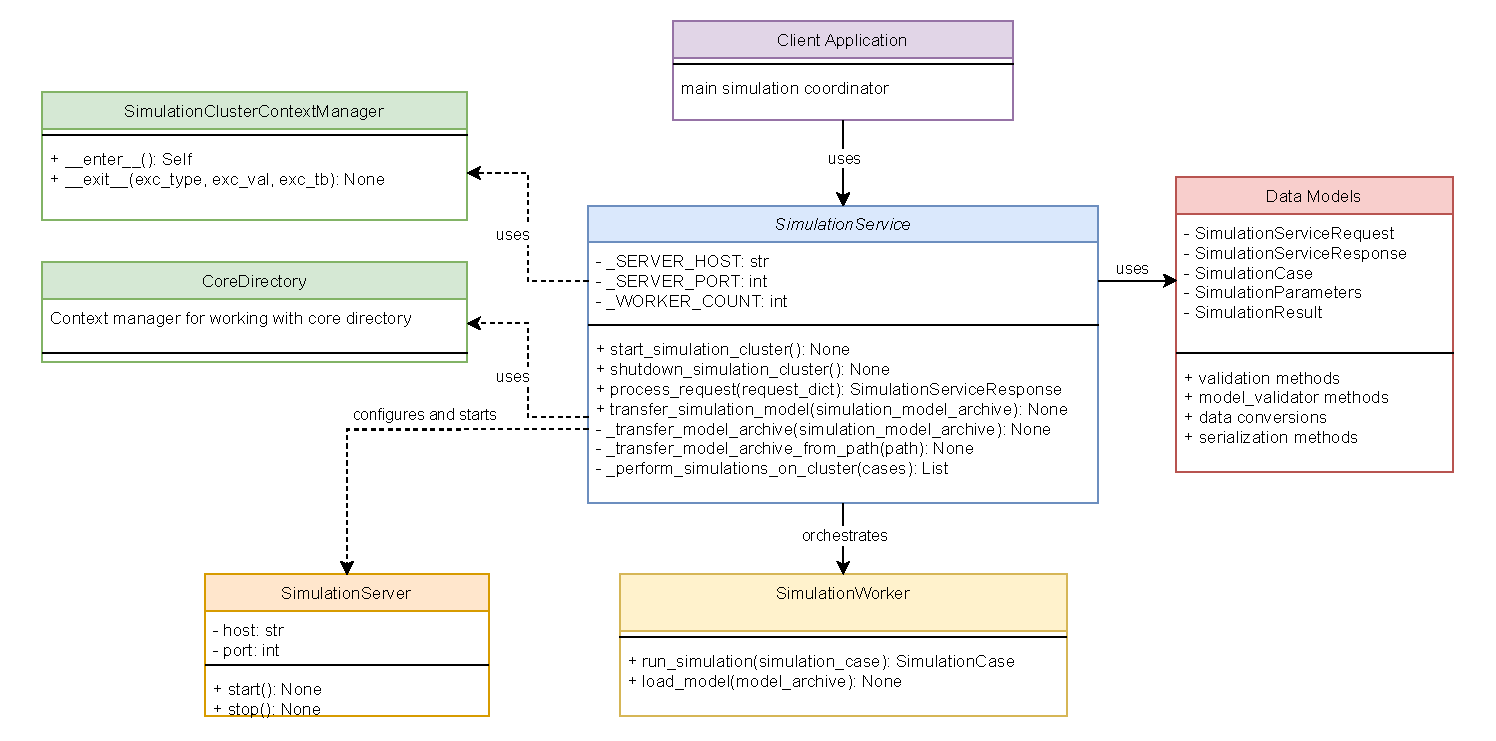
\includegraphics[width=1.0\textwidth]{content/images/SimulationServiceUML.pdf}
	\caption{Simulation service system UML}
	\label{fig:SimulationServiceUML}
\end{figure}

\textbf{Public API}
\begin{itemize}
	\item \textbf{Cluster Management}

	 \csignature{\textit{start\_simulation\_cluster() $\rightarrow$ None}}

	 Initializes and launches the simulation cluster with the configured number of worker processes.

	 \textbf{Implementation Details:}
	 \begin{itemize}
	 	\item Validates environment configuration
	 	\item Starts the gRPC server on the configured host and port
	 	\item Initializes the worker pool with \texttt{\_WORKER\_COUNT} workers
	 	\item Establishes communication channels between server and workers
	 	\item Performs health checks to ensure cluster readiness
	 \end{itemize}

	 \textbf{Thread Safety:} Thread-safe, but should not be called concurrently with \texttt{shutdown\_simulation\_cluster()}

	 \textbf{Error Handling:} Raises exceptions for configuration issues, network failures, or resource allocation problems

	\csignature{\textit{shutdown\_simulation\_cluster() $\rightarrow$ None}}

	Safely terminates the simulation cluster and releases all resources.
	\textbf{Implementation Details:}
	\begin{itemize}
		\item Gracefully shuts down active simulation tasks
		\item Releases worker processes
		\item Closes network connections
		\item Cleans up temporary files and resources
	\end{itemize}

	\textbf{Thread Safety:} Thread-safe, but should not be called concurrently with \texttt{start\_simulation\_cluster()}

	\textbf{Error Handling:} Logs errors during shutdown but attempts to complete the process regardless of failures

	\item \textbf{Simulation Execution}

	\csignature{\textit{process\_request(request)}}

	Processes a simulation request by distributing tasks to the worker pool and aggregating results.

	\textbf{Parameters:}
	\begin{itemize}
		\item \texttt{request}: A simulation request object containing parameters and configuration for the simulation
	\end{itemize}

	\textbf{Returns:}
	\begin{itemize}
		\item Processed simulation results based on the request type
	\end{itemize}

	\textbf{Implementation Details:}
	\begin{itemize}
		\item Validates and normalizes the request
		\item Determines optimal task distribution strategy
		\item Distributes tasks to worker processes
		\item Monitors execution and handles failures
		\item Aggregates and post-processes results
	\end{itemize}

	\textbf{Thread Safety:} Thread-safe, can be called concurrently

	\textbf{Error Handling:} Returns error details for invalid requests, worker failures, or timeout issues

	\item \textbf{Model Management}

	\csignature{transfer\_simulation\_model(model)}

	Prepares and transfers a simulation model to all worker nodes in the cluster via simulation server.

	\textbf{Parameters:}
	\begin{itemize}
		\item \texttt{model}: The simulation model to distribute to the cluster
	\end{itemize}

	\textbf{Implementation Details:}
	\begin{itemize}
		\item Serializes the model into an appropriate format
		\item Compresses and optimizes the model for network transfer
		\item Distributes the model to all workers in the cluster
		\item Verifies successful model installation on each worker
	\end{itemize}

	\textbf{Thread Safety:} Thread-safe, but performance may degrade with concurrent transfers

	\textbf{Error Handling:} Raises exceptions for serialization failures, network issues, or worker-side installation problems

\end{itemize}

\textbf{Data Models Schema}

The \texttt{SimulationService} uses a well-defined set of data models for handling simulation requests, cases, and results. Understanding these models is essential for effectively using the service.

\begin{figure}[H]
	\begin{lstlisting}[language=Python, caption={SimulationResults Model}]
		class SimulationResults(BaseModel):
		"""
		Container for simulation calculation results.

		Contains heat results that may be represented in various formats:
		- Single value
		- Sequence of values
		- Matrix (sequence of sequences)

		Note: This implementation aligns with SimulationResultType
		and SimulationResults from common.py
		"""
		Heat: float | Sequence[float] | Sequence[Sequence[float] | float]
	\end{lstlisting}
\end{figure}

\begin{figure}[H]
	\begin{lstlisting}[language=Python, caption={SimulationCase Model}]
		class SimulationCase(BaseModel):
		"""
		Represents a single simulation case with inputs and optional results.

		Attributes:
		wells: Well configuration data from the WellManagement service
		control_vector: Dictionary mapping control parameters to their values
		results: Optional field containing simulation results when completed
		"""
		wells: WellManagementServiceResult
		control_vector: dict[str, float]
		results: SimulationResults | None = Field(default=None)
	\end{lstlisting}
\end{figure}

\begin{figure}[H]
	\begin{lstlisting}[language=Python, caption={SimulationServiceRequest Model}]
		class SimulationServiceRequest(BaseModel):
		"""
		Container for a batch of simulation cases to be processed.

		Attributes:
		simulation_cases: List of simulation cases to be executed
		"""
		simulation_cases: list[SimulationCase]
	\end{lstlisting}
\end{figure}

\begin{figure}[h]
	\begin{lstlisting}[language=Python, caption={SimulationServiceResponse Model}]
		class SimulationServiceResponse(BaseModel):
		"""
		Container for processed simulation cases with results.

		Attributes:
		simulation_cases: List of simulation cases with populated results
		"""
		simulation_cases: list[SimulationCase]
	\end{lstlisting}
\end{figure}

\textbf{Shared models:}
\begin{enumerate}
	\item Well Management Service Models

	The SimulationService integrates with the Well Management Service through a set of shared models that define well configurations, trajectories, and completions. These models provide the foundation for simulation cases.

	\begin{figure}[H]
		\begin{lstlisting}[language=Python, caption={SimulationWellPerforation Model}]
			class SimulationWellPerforationModel(BaseModel):
			"""
			Represents a perforation in a well with a depth range and 3D coordinate points.

			Attributes:
			range: Tuple defining the start and end depths of the perforation
			points: Collection of 3D points (x,y,z) defining the perforation geometry

			Validation:
			Ensures the start depth is less than the end depth
			"""
			range: tuple[float, float]
			points: tuple[tuple[float, float, float], ...]
		\end{lstlisting}
	\end{figure}

	\begin{figure}[H]
		\begin{lstlisting}[language=Python, caption={imulationWellCompletio nModel}]
			class SimulationWellCompletionModel(BaseModel):
			"""
			Represents the completion details of a well, containing perforations.

			Attributes:
			perforations: Collection of perforation models defining the well's
			completion design
			"""
			perforations: tuple[SimulationWellPerforationModel, ...]
		\end{lstlisting}
	\end{figure}

	\begin{figure}[H]
		\begin{lstlisting}[language=Python, caption={SimulationWell Model}]
			class SimulationWellModel(BaseModel):
			"""
			Represents a complete well with identifying information, trajectory,
			and optional completion data.

			Attributes:
			name: Unique identifier for the well
			trajectory: Collection of 3D points (x,y,z) defining the well path
			completion: Optional completion details for the well
			"""
			name: str
			trajectory: tuple[tuple[float, float, float], ...]
			completion: SimulationWellCompletionModel | None = Field(default=None)
		\end{lstlisting}
	\end{figure}

	\begin{figure}[H]
		\begin{lstlisting}[language=Python, caption={WellManagementServiceResult Model}]
			class WellManagementServiceResult(BaseModel):
			"""
			Container for the results from the Well Management Service,
			providing a collection of well models for simulation.

			Attributes:
			wells: List of well models to be used in simulation

			Validation:
			Ensures all well names are unique within the collection
			"""
			wells: list[SimulationWellModel]
		\end{lstlisting}
	\end{figure}

	The well management models form a hierarchical structure:

	\begin{itemize}
		\item \textbf{WellManagementServiceResult} contains multiple \textbf{SimulationWellModel} objects
		\item Each \textbf{SimulationWellModel} contains:
		\begin{itemize}
			\item A unique name identifier
			\item A trajectory defined as a sequence of 3D points
			\item Optional \textbf{SimulationWellCompletionModel}
		\end{itemize}
		\item \textbf{SimulationWellCompletionModel} contains multiple \textbf{SimulationWellPerforationModel} objects
		\item Each \textbf{SimulationWellPerforationModel} contains:
		\begin{itemize}
			\item A depth range defined as (start, end)
			\item A collection of 3D points defining perforation geometry
		\end{itemize}
	\end{itemize}
\end{enumerate}

\bigskip

The models form a hierarchical structure:

\begin{itemize}
	\item \textbf{SimulationServiceRequest} contains multiple \textbf{SimulationCase} objects
	\item Each \textbf{SimulationCase} contains:
	\begin{itemize}
		\item Well configuration data (\textbf{WellManagementServiceResult})
		\item Control parameters as a dictionary
		\item Optional \textbf{SimulationResults} (null on input, populated on output)
	\end{itemize}
	\item \textbf{SimulationResults} contains heat data in various formats
\end{itemize}




\textbf{Detailed Workflow}
\begin{enumerate}
	\item Cluster Initialization
	\begin{itemize}
		\item Triggered via docker-compose up.
		\item Instantiates:
		\begin{itemize}
			\item One server container
			\item A configurable number of worker containers
		\end{itemize}
		\item Workers automatically attempt to connect to the server upon initialization.
	\end{itemize}
	\item Simulation Model Distribution:
	\begin{itemize}
		\item Once workers are running, they attempt to request the simulation model via gRPC.
		\item Server checks if the model has already been uploaded:
		\begin{itemize}
			\item If not uploaded, the server responds with a "model not available" status. Workers enter a wait/retry loop.
			\item Once a model is uploaded, the server sends a model archive to each requesting worker.
		\end{itemize}
		\item Upon receiving the archive, each worker:
		\begin{itemize}
			\item Unpacks and locally stores the simulation model.
			\item Becomes ready to accept simulation jobs
		\end{itemize}
	\end{itemize}
	\item Simulation Job Dispatching
	\begin{itemize}
		\item With the model in place, workers begin polling the server for simulation jobs
		\item Server responses can include:
		\begin{itemize}
			\item "No jobs available": Worker waits before retrying.
			\item "New job available": Server sends a new simulation case as the payload.
		\end{itemize}
		\item Each simulation case contains:
		\begin{itemize}
			\item Well configurations - results of WellManagementService.
			\item A control vector with simulation parameters - just to keep closely optimization configuration and simulation results, as worker can pull simulation case in any order.
			\item A placeholder for results.
		\end{itemize}
	\end{itemize}
	\item Job Execution and Result Submission
	\begin{itemize}
		\item Upon receiving a job, the worker executes the simulation using the local model and the provided input data.
		\item Once complete, the worker submits the completed simulation case back to the server, now containing the computed results.
		\item Server:
		\begin{itemize}
			\item Acknowledges receipt.
			\item Updates internal tracking of job progress and worker status.
		\end{itemize}
		\item This loop continues until all jobs are processed.
	\end{itemize}
	\item Cluster Shutdown
	\begin{itemize}
		\item The system is terminated with docker-compose down, which:
		\begin{itemize}
			\item Shuts down all running containers (server and workers).
			\item Cleans up associated Docker resources.
		\end{itemize}
		\item All operations cease gracefully, preserving simulation state up to the point of shutdown.
	\end{itemize}
\end{enumerate}

\bigskip
\textbf{Dependencies}

\begin{itemize}
	\item gRPC framework for communication
	\item Protobuf for data serialization
	\item Numpy/SciPy for numerical operations
	\item Logging framework for operational monitoring
\end{itemize}

\bigskip
\textbf{Supported simulators}:
\begin{itemize}
	\item OpenDarts
\end{itemize}
